\chapter{Noise Filtering}\label{NoiseFiltering}
\section{Research}
\subsection{Voice frequency analysis}
\paragraph{} Voice frequency ranges vary heavily depending on whether it sources from a male of a female. Fundamental voice frequency varies from 100Hz to 900 Hz for men and 350Hz to 3KHz for women. Including peaks to conserve natural sounding voice, a wider frequency range has to be considered. It rises to 8 KHz for males and 17KHz for females \cite{Seaindia}. Yet different researches often come up with different results. For example, in phone communications it is accepted to transmit frequency range between 400Hz and 3400Hz. This is the reason some peoples' voices transit poorly over the phone yet for most cases it work fine. This example allows to conclude that smaller frequency ranges could be acceptable. To conserve all of the properties of the human voice, filter boundaries should be around 100Hz to 17KHz but this range would most likely not  filter out any noise as it takes up almost an entire frequency range of human hearing (approximately 20Hz to 20KHz).  
\subsection{Filter characteristics}
\paragraph{} Firstly it was defined that the input response of the signal is infinite and therefore an IIR filter has to be applied. Considering that computing power limitation is out of scope for this project, it was decided to use Butterworth filter as around higher orders of this filter type it approaches rectangular form (an ideal filter).  
\section{Results}
\paragraph{} Making a field research to find the frequency range that would fit the needs of this project was out scope, therefore to test the filters it was decided to take trial-error approach. A few samples were made outside during a windy day. This was considered a good idea as it has recreated one of the most common conversation scenarios.
\paragraph{} At first it was attempted to conserve the entire frequency range that humans can produce. This has resulted in a filter that seemed to filter out a big part of the noise but if it was listened to, all of the previously recorded noise was still there.It was hard to tell the difference between filtered and not filtered sound samples.

\begin{figure}[htp]
  \centering
    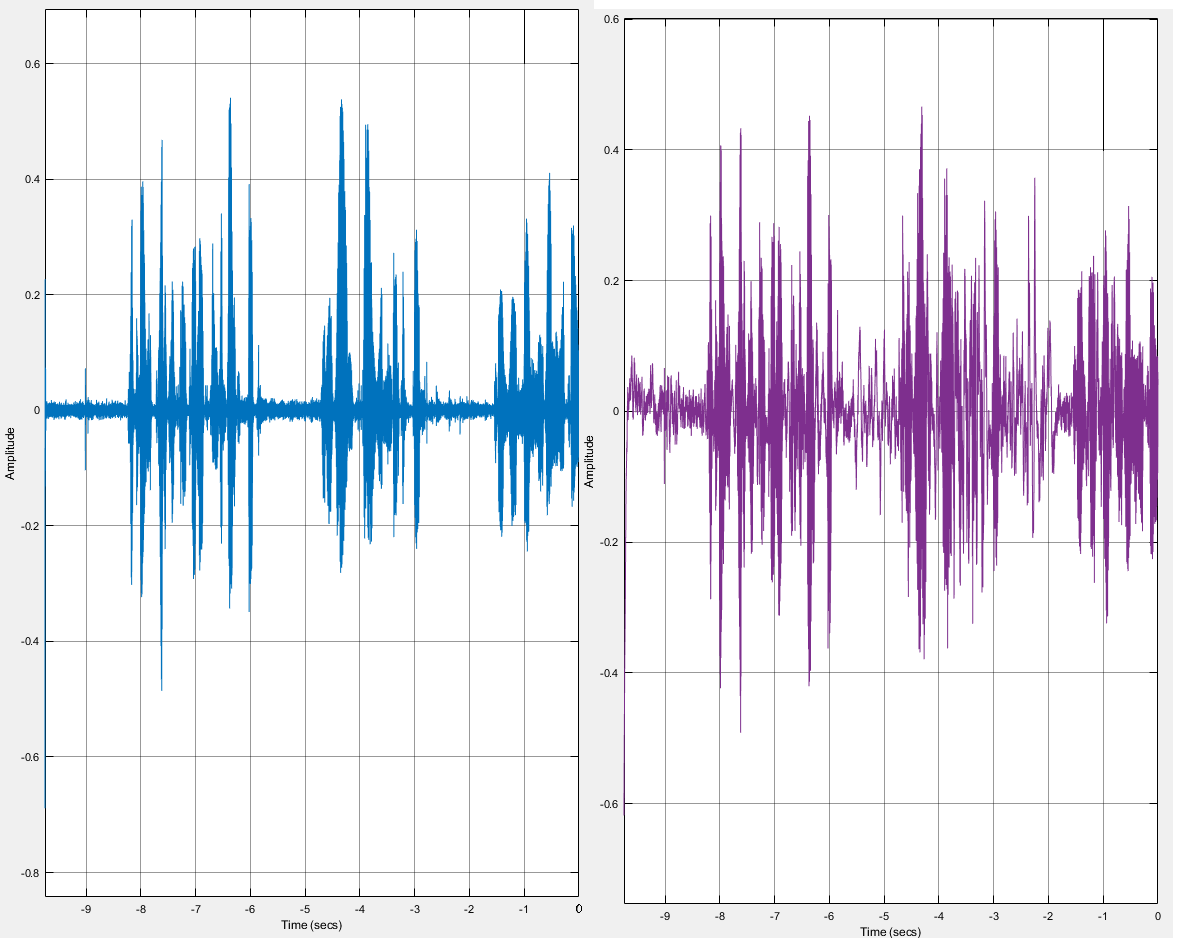
\includegraphics[width=0.7\paperwidth]{Illustrations/100HZto17KHzfilter}
    \caption{Recorded sample on the right and filtered result on the left}
\end{figure}

\paragraph{} As the first approach did not seem to output a satisfying result, it was attempted to the signals by leaving only fundamental frequency radius (100Hz to 3KHz. The result seemed to be far more satisfying as most of the noise was eliminated. However, output clarity was poorer by far in comparison to original. Result of this test could be considered a solution for noise canceling although it would be a very poor one.

\begin{figure}
  \centering
    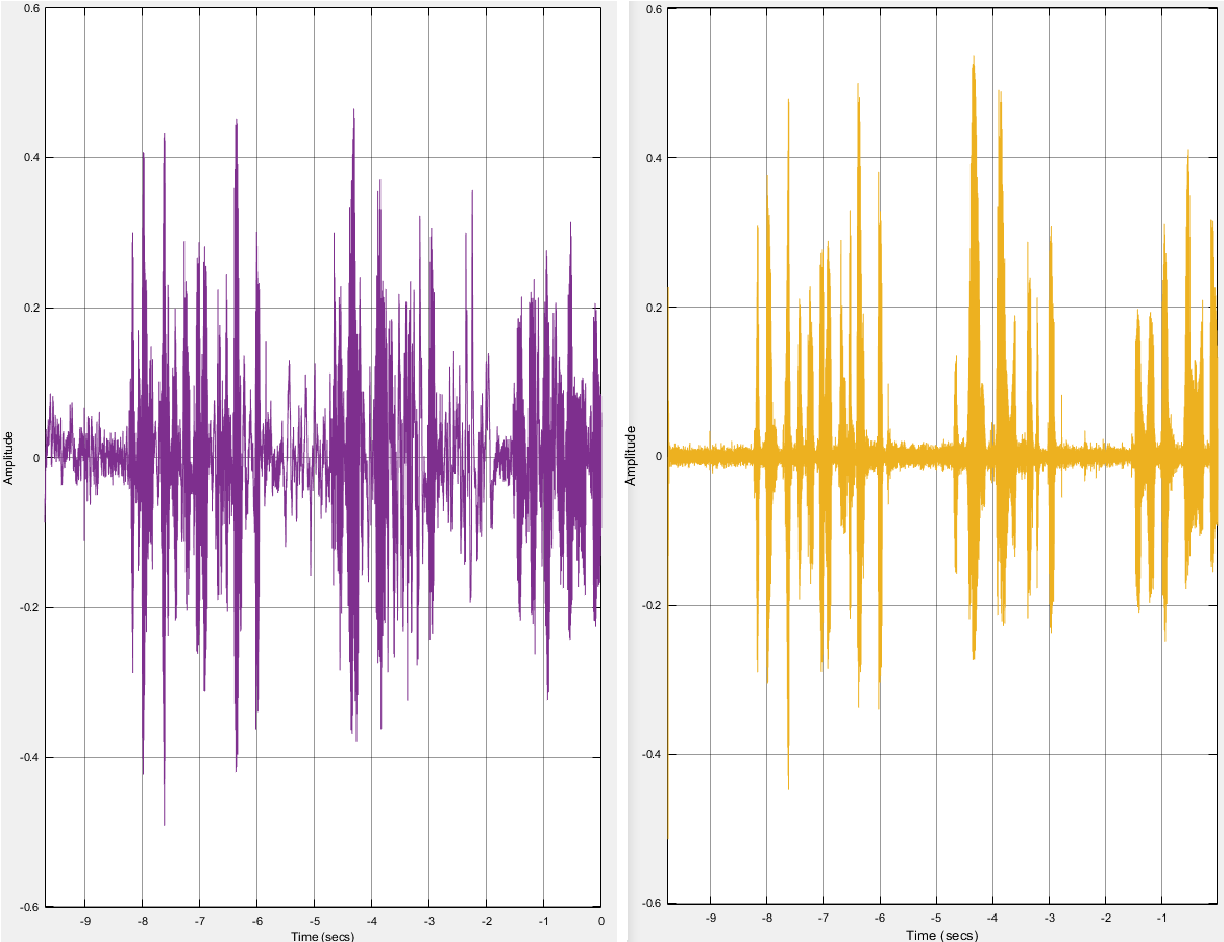
\includegraphics[width=0.7\paperwidth]{Illustrations/100HZto3KHzfilter}
    \caption{Recorded sample on the right and filtered result on the left}
\end{figure}

\paragraph{} Finally the frequency range picked for communication through phone (400Hz to 3400Hz) was taken to trial. Output of the filter was barely different when compared to one the previous one. It had filtered out most of the noise yet the sound clarity was still very poor.

\begin{figure}[htp]
  \centering
    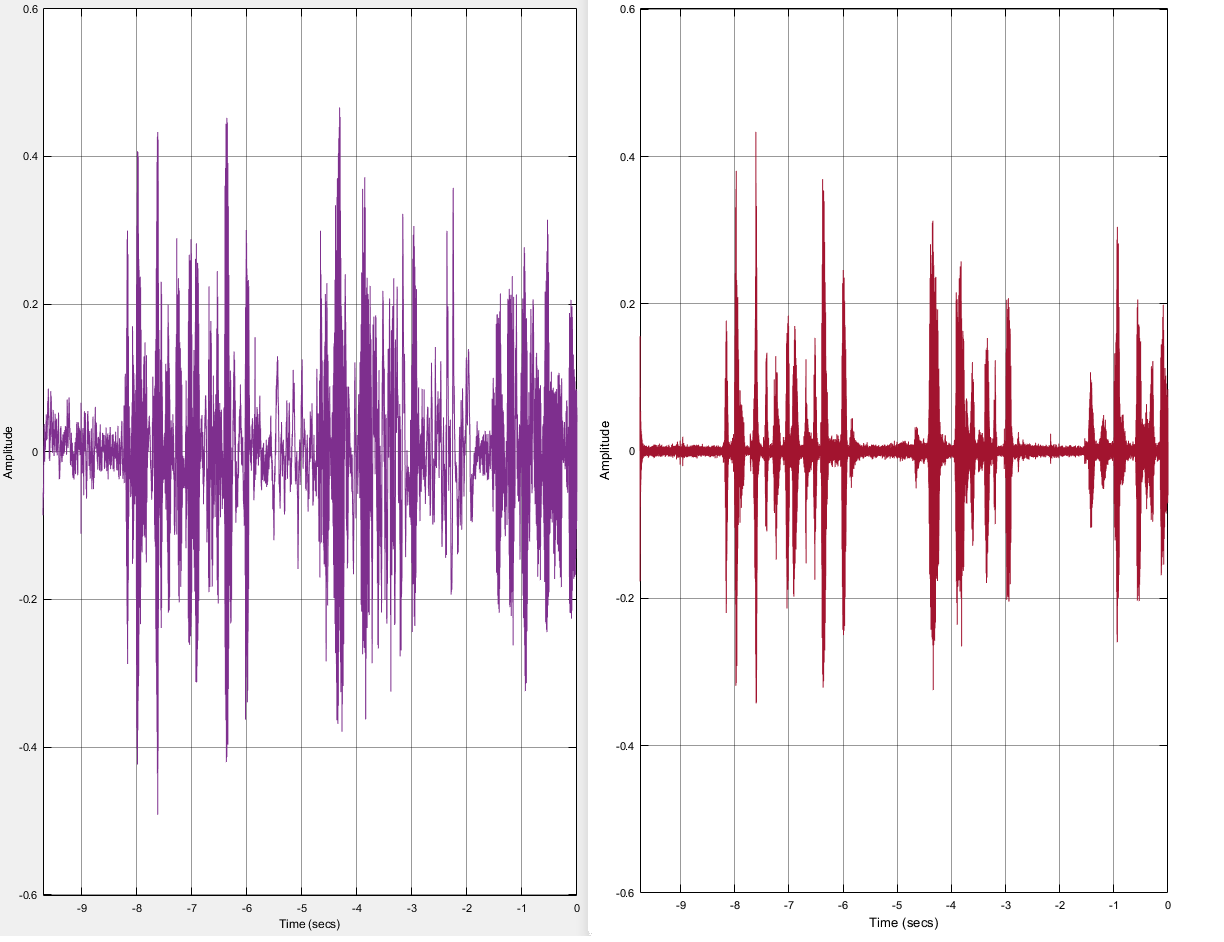
\includegraphics[width=0.7\paperwidth]{Illustrations/400HZto3400Hzfilter}
    \caption{Recorded sample on the right and filtered result on the left}
\end{figure}

\section{Conclusion}
\paragraph{} The approach that the group has taken seems to be correct - the filters worked as intended, however a question was raised whether this method is capable of producing a signal that would cancel out most of the sound without affecting sound quality. The filter could be more efficient if different frequency ranges were available to pick from to filter out noises that are common in different environments. This would require in-depth analysis of noises in these environments.  


  